% !TeX spellcheck = fr_FR
\chapter{Chapitre 12: Déploiement et Conteneurisation}
\label{chap:deploiement}

Ce chapitre présente la conteneurisation du projet, conçue pour un déploiement automatisé. Une seule commande initialise la base de données, exécute les scripts d'importation et lance l'application web sur \texttt{http://localhost:5001}.

Nous détaillerons le rôle des fichiers \texttt{dockerfile}, \texttt{docker-compose.yml}, \texttt{entrypoint.sh} et \texttt{.dockerignore}.

\section{Introduction à Docker}
Docker est une plateforme open-source qui automatise le déploiement, la mise à l'échelle et la gestion des applications en utilisant la conteneurisation\citeref{ref:docker_docs}. Un conteneur est une unité logicielle légère et autonome qui inclut tout ce dont une application a besoin pour fonctionner : le code, les dépendances, les bibliothèques et les outils système. 

Contrairement aux machines virtuelles qui virtualisent un système d'exploitation complet, les conteneurs partagent le noyau de l'hôte tout en maintenant l'isolation des processus. Cette approche offre plusieurs avantages: démarrage rapide (quelques secondes), empreinte mémoire réduite, et portabilité accrue. Les conteneurs isolent les applications les unes des autres et de leur environnement, garantissant ainsi qu'elles fonctionnent de manière cohérente sur n'importe quelle infrastructure supportant Docker.

\subsectionsection{Pourquoi dockeriser ?}

Trois raisons concrètes :
\begin{itemize}
  \item \textbf{Reproductibilité}: même version de Python, mêmes dépendances système (\texttt{wkhtmltopdf}\citeref{ref:wkhtmltopdf}, client MySQL), même environnement d'exécution.
  \item \textbf{Parité dev/prod}: une pile unique (app + base) réduisant les \og ça marche sur ma machine\fg{}.
  \item \textbf{Bootstrap instantané}: une commande pour installer, migrer, télécharger/traiter les données et lancer le serveur.
\end{itemize}

\section{Les quatre pièces du puzzle}

\begin{description}
  \item[\texttt{dockerfile}] Image de l'application: base Python 3.9 \texttt{slim-bookworm}, dépendances \textit{apt}, \texttt{pip}, copie du code et \texttt{ENTRYPOINT}.
  \item[\texttt{docker-compose.yml}] Orchestration multi-services: \texttt{db} (MySQL) + \texttt{app} et \texttt{app-dev} (profils), volumes, variables d'environnement\citeref{ref:docker_compose_env_vars}, \texttt{depends\_on} avec healthcheck.
  \item[\texttt{entrypoint.sh}] Orchestrateur de démarrage côté \texttt{app}: attend MySQL, applique migrations, exécute scripts de données (selon flags), lance Flask.
  \item[\texttt{.dockerignore}] Réduit le contexte de build (ignore les dossiers volumineux et la documentation), accélère et assainit l'image.
\end{description}


\begin{figure}[H]
  \centering
  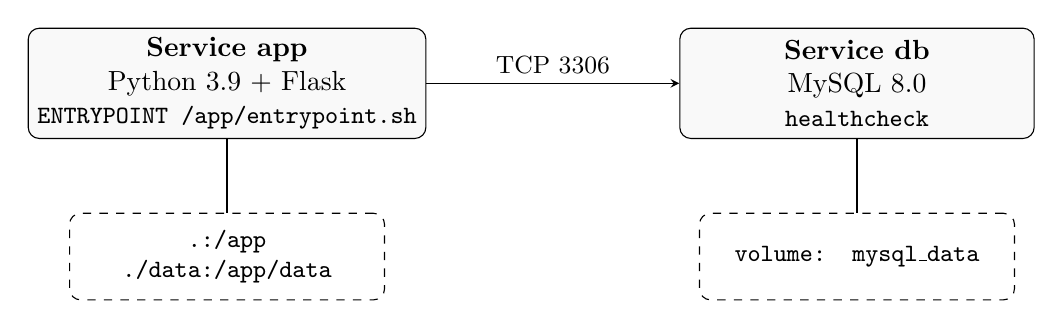
\begin{tikzpicture}[node distance=2.5cm, >=stealth]
    \tikzstyle{svc}=[draw, rounded corners, minimum width=4.5cm, minimum height=1.4cm, align=center, fill=gray!5]
    \tikzstyle{vol}=[draw, dashed, rounded corners, minimum width=4cm, minimum height=1.1cm, align=center, font=\small]

    \node[svc] (app) {\textbf{Service app}\\ Python 3.9 + Flask\\ \small \texttt{ENTRYPOINT /app/entrypoint.sh}};
    \node[svc, right of=app, node distance=8cm] (db) {\textbf{Service db}\\ MySQL 8.0\\ \small \texttt{healthcheck}};
    \node[vol, below of=db, node distance=2.2cm] (mysqlvol) {\texttt{volume: mysql\_data}};
    \node[vol, below of=app, node distance=2.2cm] (codevol) {\texttt{.:/app}\\ \texttt{./data:/app/data}};

    \draw[->] (app) -- node[above]{\small TCP 3306} (db);
    \draw[-] (db) -- (mysqlvol);
    \draw[-] (app) -- (codevol);
  \end{tikzpicture}
  \caption{Deux conteneurs reliés sur le réseau compose; volumes pour le code (monté) et les données MySQL (persistées).}
\end{figure}

\section{L'orchestration: \texttt{docker-compose.yml}}

Le fichier compose\citeref{ref:docker_compose} définit \texttt{db}, \texttt{app} et un service \texttt{app-dev} activé via profil. Extraits commentés:

\begin{codebox}{\texttt{db} : MySQL 8.0 avec healthcheck}
services:
  db:
    image: mysql:8.0
    environment:
      MYSQL_ROOT_PASSWORD: root
      MYSQL_DATABASE: stops_db
      MYSQL_USER: stops_user
      MYSQL_PASSWORD: 1234
    ports:
      - "3306:3306"
    volumes:
      - mysql_data:/var/lib/mysql
    healthcheck:
      test: ["CMD-SHELL", "mysqladmin ping -h localhost -u$${MYSQL_USER} -p$${MYSQL_PASSWORD}"]
      interval: 10s
      timeout: 5s
      retries: 2
\end{codebox}

\noindent L'application dépend explicitement du statut \textit{healthy} de MySQL\citeref{ref:mysql_docs} et monte deux volumes (code + données):

\begin{codebox}{\texttt{app} : service principal}
  app:
    build: .
    ports:
      - "5001:5001"
    volumes:
      - .:/app
      - ./data:/app/data
    depends_on:
      db:
        condition: service_healthy
    environment:
      # Variables lues depuis .env si présentes (avec valeurs par défaut)
      MYSQL_USER: ${MYSQL_USER:-stops_user}
      MYSQL_PASSWORD: ${MYSQL_PASSWORD:-1234}
      AUTH_DB_USER: ${AUTH_DB_USER:-}
      AUTH_DB_PASSWORD: ${AUTH_DB_PASSWORD:-}
      DATABASE_URI: ${DATABASE_URI:-mysql+pymysql://stops_user:1234@db/stops_db}
      AUTH_DATABASE_URI: ${AUTH_DATABASE_URI:-mysql+pymysql://stops_user:1234@db/auth_db}
      AUTO_MIGRATE: "true"
      MATCH_ONLY: "${MATCH_ONLY:-false}"
      SECRET_KEY: ${SECRET_KEY:-dev-insecure}
\end{codebox}

\noindent Pour developer l'application web, nous activons un service plus léger qui évite les téléchargements et prétraitements longs:

\begin{codebox}{\texttt{app-dev} : profil \texttt{dev}}
  app-dev:
    profiles: [dev]
    build: .
    volumes:
      - .:/app
      - ./data:/app/data
    environment:
      SKIP_DATA_IMPORT: "true"
      AUTO_MIGRATE: "true"
\end{codebox}

\section{L'image: \texttt{dockerfile}}

L'image part d'un Python 3.9 minimal \texttt{slim-bookworm} (compatibilité \texttt{wkhtmltopdf}). Nous installons plusieurs dépendances système critiques: \texttt{wkhtmltopdf} pour la génération PDF, \texttt{default-mysql-client} pour les commandes d'administration MySQL, \texttt{dos2unix} pour normaliser les fins de lignes, et les bibliothèques GDAL/GEOS nécessaires à GeoPandas pour le traitement géospatial. Puis \texttt{pip install -r requirements.txt} et utilisation d'un \texttt{ENTRYPOINT} shell.

\begin{codebox}[language=bash]{Extraits — \texttt{dockerfile} (utilisateur non-root)}
FROM python:3.9-slim-bookworm
ENV FLASK_APP=backend/app.py \\
    FLASK_RUN_HOST=0.0.0.0 \\
    FLASK_RUN_PORT=5001
RUN apt-get update && apt-get install -y --no-install-recommends \\
    wkhtmltopdf default-mysql-client dos2unix && rm -rf /var/lib/apt/lists/*

# Crée un utilisateur non-root configurable
ARG APP_UID=1000
ARG APP_GID=1000
RUN groupadd -g ${APP_GID} app && \\
    useradd -m -u ${APP_UID} -g ${APP_GID} -s /bin/bash app

WORKDIR /app
COPY requirements.txt /app/
RUN pip install --no-cache-dir -r requirements.txt
COPY entrypoint.sh /app/entrypoint.sh
RUN dos2unix /app/entrypoint.sh && chmod +x /app/entrypoint.sh
COPY . /app/

# Permissions minimales et répertoires d'écriture
RUN find /app -type d -exec chmod 755 {} \; && \\
    find /app -type f -exec chmod 644 {} \; && \\
    chmod 755 /app/entrypoint.sh && \\
    mkdir -p /app/data /app/.cache && \\
    chown -R app:app /app && \\
    chmod 775 /app/data /app/.cache

# Exécute en tant qu'utilisateur non-root
USER app

EXPOSE 5001
ENTRYPOINT ["/bin/bash", "/app/entrypoint.sh"]
\end{codebox}

\section{Le chef d'orchestre: \texttt{entrypoint.sh}}

Le script d'entrée synchronise le démarrage: attend MySQL, crée la base \texttt{auth\_db} si besoin, applique les migrations, exécute les scripts de données (selon les drapeaux), puis lance Flask\citeref{ref:flask_docs}. Il peut également créer un utilisateur dédié pour \texttt{auth\_db} si des variables d'environnement sont fournies.

\begin{codebox}[language=bash]{Attente active, création de comptes, migrations}
echo "Waiting for MySQL database at db:3306..."
while ! mysqladmin ping -h"db" -P3306 --silent \\
        --user=${MYSQL_USER} --password=${MYSQL_PASSWORD}; do
    sleep 1
done
echo "MySQL is up and ready."

if [ -n "$MYSQL_ROOT_PASSWORD" ]; then
  # Assure l'existence de auth_db et droits de base
  mysql -h db -uroot -p"${MYSQL_ROOT_PASSWORD}" -e "
    CREATE DATABASE IF NOT EXISTS auth_db 
      CHARACTER SET utf8mb4 COLLATE utf8mb4_unicode_ci;
    GRANT ALL PRIVILEGES ON auth_db.* TO 'stops_user'@'%';
    FLUSH PRIVILEGES;" || true
  
  # Crée un utilisateur dédié auth si variables fournies
  if [ -n "$AUTH_DB_USER" ] && [ -n "$AUTH_DB_PASSWORD" ]; then
    mysql -h db -uroot -p"${MYSQL_ROOT_PASSWORD}" -e "
      CREATE USER IF NOT EXISTS '${AUTH_DB_USER}'@'%' 
        IDENTIFIED BY '${AUTH_DB_PASSWORD}';
      GRANT SELECT, INSERT, UPDATE, DELETE, CREATE, ALTER, INDEX 
        ON auth_db.* TO '${AUTH_DB_USER}'@'%';
      REVOKE ALL PRIVILEGES ON auth_db.* FROM 'stops_user'@'%';
      FLUSH PRIVILEGES;" || true
  fi
fi

if [ "${AUTO_MIGRATE:-false}" = "true" ]; then
  [ ! -d "migrations" ] && flask db init || true
  flask db migrate -m "Auto migration" || true
fi
flask db upgrade || true
\end{codebox}

\noindent Le démarrage exécute également \texttt{create\_auth\_tables.py} pour s'assurer que le schéma \texttt{auth\_db} inclut \textbf{\texttt{users}} et \textbf{\texttt{auth\_events}} (journalisation d'audit).

\section{Démarrer en 30 secondes}

\begin{cmdbox}
docker compose up -d
\end{cmdbox}

\noindent Attendez quelques secondes; l'app est disponible sur \texttt{http://localhost:5001}. Pour le mode développement (sans préparation de données):

\begin{cmdbox}
docker compose --profile dev up -d
\end{cmdbox}

\noindent Pour consulter les logs et vérifier que tout s'enchaîne bien:

\begin{cmdbox}
docker compose logs -f app | cat
\end{cmdbox}

\noindent Pour ne suivre que les \emph{événements d'authentification} structurés (JSON), filtrez:
\begin{cmdbox}
docker compose logs -f app | grep auth_event | cat
\end{cmdbox}

\begin{figure}[H]
  \centering
  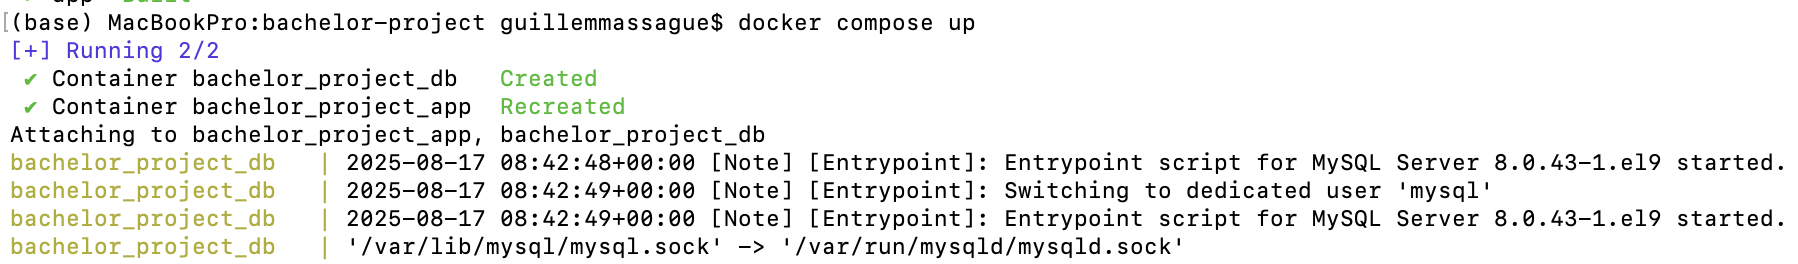
\includegraphics[width=\textwidth]{\detokenize{chap12/screenshot terminal docker compose up.png}}
  \caption{Commande et sortie de \texttt{docker compose up} dans le terminal.}
\end{figure}

\begin{figure}[H]
  \centering
  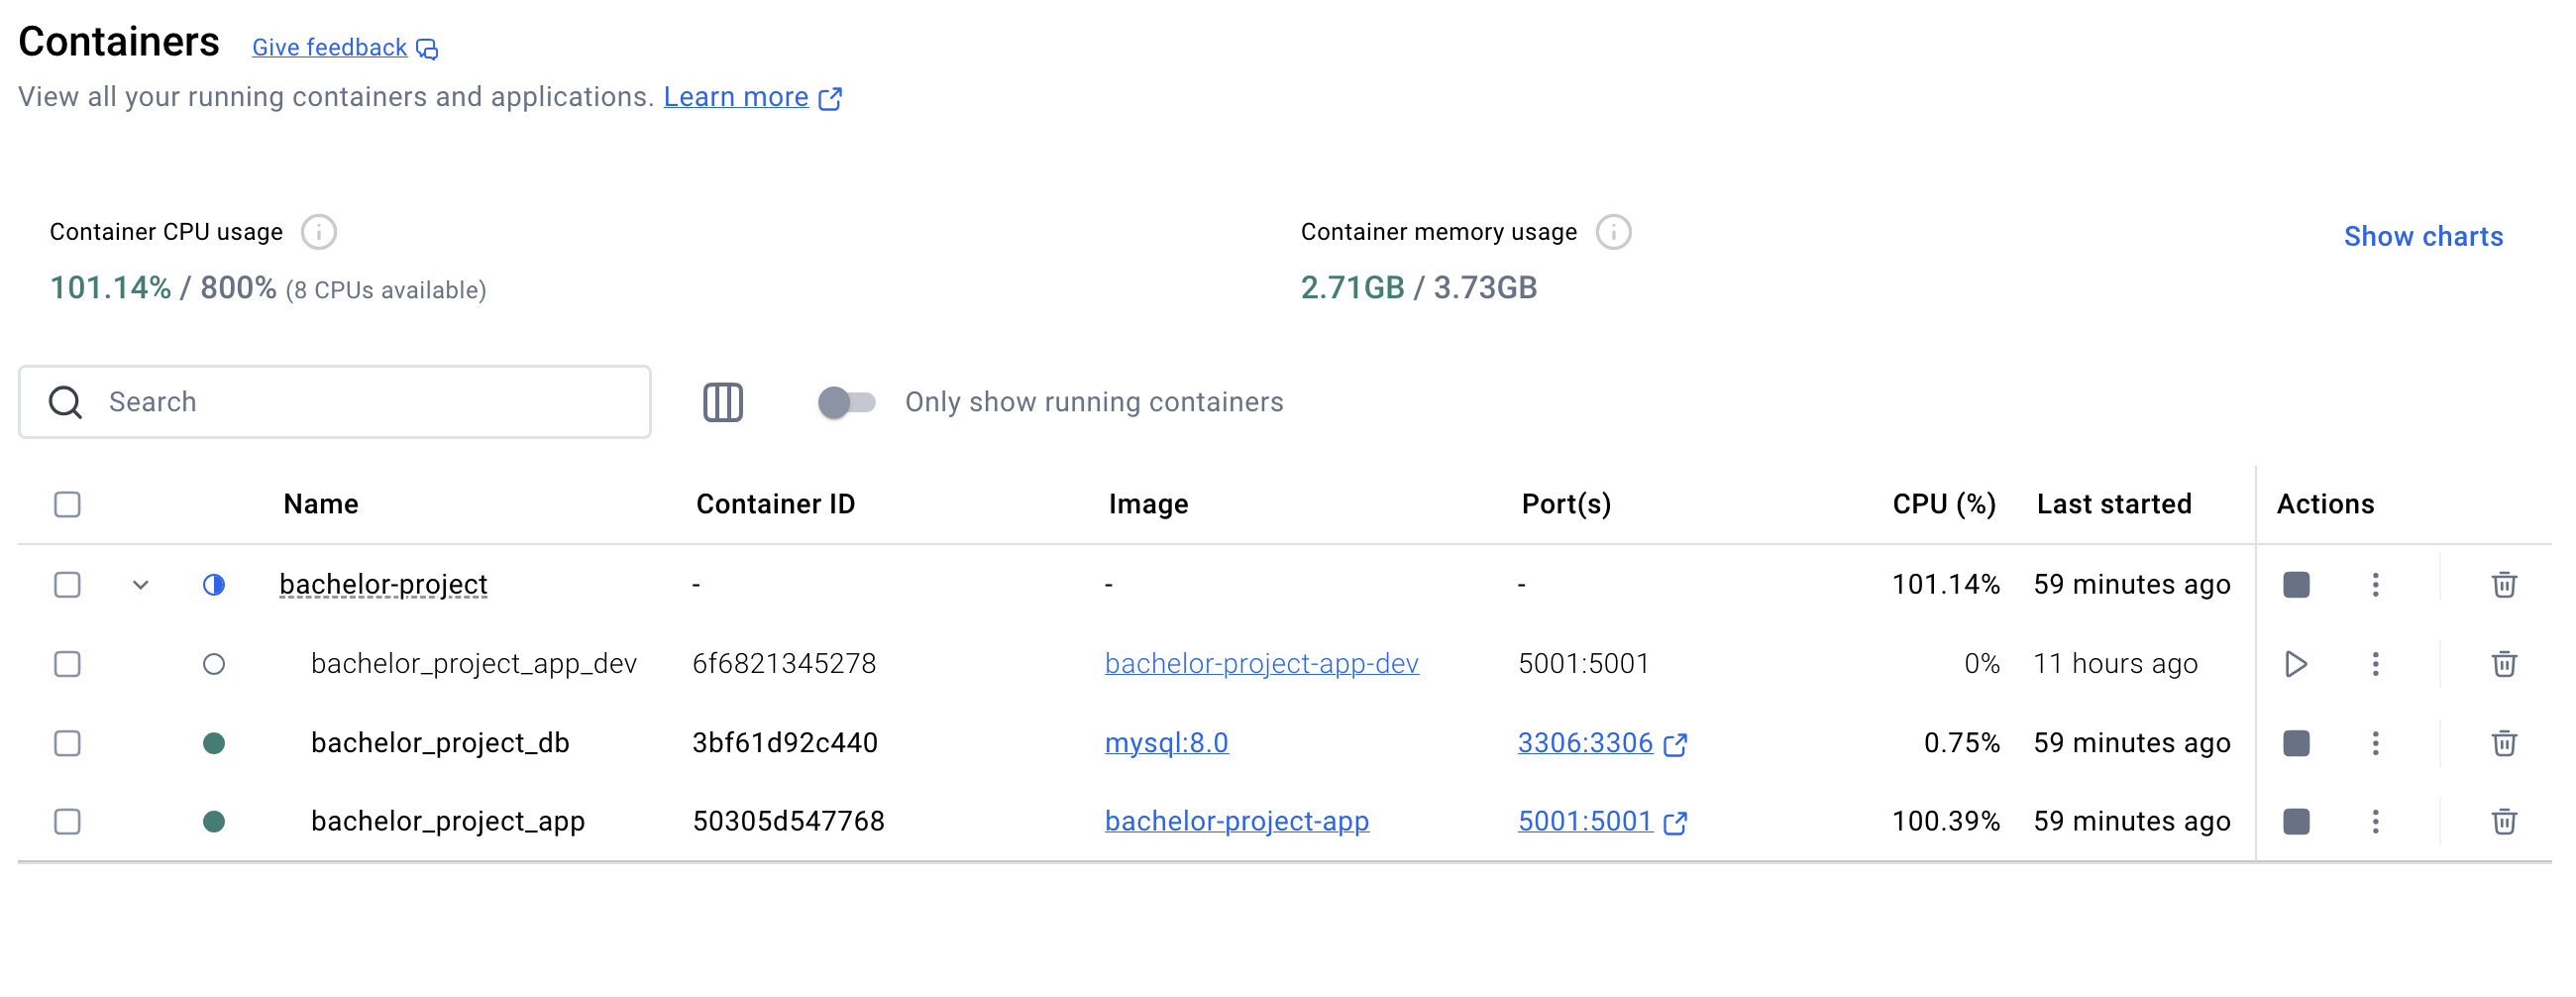
\includegraphics[width=\textwidth]{\detokenize{chap12/screenshot doker desktop.wecanseethe3containers.png}}
  \caption{Docker Desktop montrant les conteneurs en cours d'exécution.}
\end{figure}


\section{Variables d'environnement}

Les principales variables s'ajustent dans \texttt{docker-compose.yml} (ou via \texttt{.env}).

\begin{table}[H]
\centering
\caption{Variables d'environnement pour la personnalisation}
\label{tab:chap12_env_vars}
\begin{tabularx}{0.98\textwidth}{>{\raggedright\arraybackslash}p{0.25\textwidth} >{\raggedright\arraybackslash}p{0.25\textwidth} X}
\toprule
\textbf{Variable} & \textbf{Rôle} & \textbf{Valeur par défaut}\\
\midrule
\texttt{DATABASE\_URI} & Connexion MySQL (stops) & \texttt{mysql+pymysql://stops\_user:1234@db/stops\_db}\\
\texttt{AUTH\_DATABASE\_URI} & Base d'authentification & \texttt{mysql+pymysql://.../auth\_db}\\
\texttt{AUTH\_DB\_USER}, \texttt{AUTH\_DB\_PASSWORD} & Compte dédié auth (optionnel) & \texttt{\textit{vide par défaut}}\\
\texttt{AUTO\_MIGRATE} & Init/migrate auto Alembic\citeref{ref:alembic_docs} & \texttt{true} (dev)\\
\texttt{SKIP\_DATA\_IMPORT} & Sauter pipeline de données & \texttt{false} (app), \texttt{true} (app-dev)\\
\texttt{MATCH\_ONLY} & N'exécuter que matching + import & \texttt{false}\\
\texttt{FLASK\_ENV}, \texttt{FLASK\_DEBUG} & Mode Flask & \texttt{development}, \texttt{1}\\
\bottomrule
\end{tabularx}
\end{table}

\section{Persistance et poids d'image}

\textbf{Persistance MySQL.} Le volume \texttt{mysql\_data} conserve la base entre redémarrages. Vous pouvez purger pour repartir de zéro:

\begin{cmdbox}
docker compose down -v  # ATTENTION: supprime le volume mysql_data
\end{cmdbox}

\textbf{Contexte de build réduit.} Le \texttt{.dockerignore} exclut la documentation, les gros dossiers de données, les caches Python et métadonnées VCS (tout en gardant quelques fichiers essentiels pour \texttt{MATCH\_ONLY}). Cela accélère \texttt{docker build} et évite des images obèses.

\begin{codebox}[language=bash]{Extraits — \texttt{.dockerignore}}
# Métadonnées VCS et IDE
.git
.vscode/
.idea/

# Caches Python et artefacts de build
__pycache__/
*.py[cod]
*.egg-info/

# Gros dossiers de données (exclus par défaut)
data/raw/
data/processed/*
!data/processed/osm_nodes_with_routes.csv
!data/processed/atlas_routes_unified.csv

# Documentation et rapport
memoire/
documentation/
\end{codebox}

\section{Considérations de sécurité}

La conteneurisation apporte plusieurs avantages sécuritaires, mais nécessite des précautions spécifiques:

\textbf{Utilisateur non-root.} Le conteneur s'exécute sous l'utilisateur \texttt{app} (UID/GID configurables), réduisant les risques d'escalade de privilèges. Les permissions des fichiers sont minimisées (\texttt{644} pour les fichiers, \texttt{755} pour les répertoires).

\textbf{Gestion des secrets.} Les mots de passe MySQL sont passés via variables d'environnement. En production, il serait préférable d'utiliser Docker secrets\citeref{ref:docker_secrets} ou un gestionnaire externe (HashiCorp Vault, AWS Secrets Manager).

\textbf{Isolation réseau.} Les conteneurs communiquent via un réseau Docker privé. Seuls les ports explicitement exposés (\texttt{3306}, \texttt{5001}) sont accessibles depuis l'hôte.

\textbf{Surface d'attaque réduite.} L'image \texttt{slim-bookworm} contient moins de packages que l'image complète \texttt{python:3.9}. Le \texttt{.dockerignore} évite d'inclure des fichiers sensibles dans le contexte de build.




\noindent\textbf{Conclusion.} Cette dockerisation est volontairement pragmatique: peu de magie, des scripts explicites, et des profils qui servent les usages quotidiens. L'approche privilégie la lisibilité et la maintenabilité, tout en respectant les bonnes pratiques de sécurité (utilisateur non-root, isolation réseau, surface d'attaque minimale). Cette base solide facilite tant le développement local que le déploiement automatisé, et peut évoluer vers des architectures plus complexes selon les besoins.
